\documentclass[a4paper,11pt]{article}
\usepackage[utf8]{inputenc}
\usepackage[T1]{fontenc}
\usepackage{amsmath,amssymb}
\usepackage[a4paper,left=2cm,right=2cm,top=3.6cm,bottom=2.3cm,headheight=1.1cm,headsep=0.6cm,footskip=1cm]{geometry}
\usepackage{xcolor}
\usepackage{tikz}
\usetikzlibrary{calc,arrows.meta,positioning,shapes.geometric}
\usepackage{fancyhdr}
\usepackage{lastpage}
\usepackage{tabularx}
\usepackage{array}
\usepackage[most]{tcolorbox}
\usepackage{enumitem}
\usepackage{needspace}

% ---------- palet ungu tua dan jingga (Set 2) ----------
\definecolor{mainc}{HTML}{4A2C7A}
\definecolor{accc}{HTML}{E08A0B}
\definecolor{deepc}{HTML}{2D1B4E}
\definecolor{softbg}{HTML}{F5F0FA}
\definecolor{warmc}{HTML}{138D90}
\newcommand{\dis}{\displaystyle}
\newcommand{\sm}[1]{\left[\begin{smallmatrix}#1\end{smallmatrix}\right]}
\newcommand{\tr}{\operatorname{tr}}

\setlength{\parindent}{0pt}
\renewcommand{\arraystretch}{1.35}

\tikzset{
  ar/.style={-{Stealth[length=1.8mm]},thick,mainc},
  nd/.style={circle,draw=mainc,thick,fill=softbg,minimum size=6mm,inner sep=0pt,font=\scriptsize}
}

% ---------- header ----------
\pagestyle{fancy}
\fancyhf{}
\renewcommand{\headrulewidth}{0pt}
\fancyhead[L]{%
  \begin{tikzpicture}[remember picture,overlay]
    \fill[mainc] ([yshift=-1.2cm]current page.north west) rectangle ([yshift=-3.15cm]current page.north east);
    \fill[accc] ([yshift=-3.15cm]current page.north west) rectangle ([yshift=-3.25cm]current page.north east);
  \end{tikzpicture}%
  \color{white}\bfseries\large Latihan Soal Matriks (Set 2)}
\fancyhead[R]{\color{white}\small Diunduh dari website \textbf{Math1729}\ \,|\,\ 5 Oktober 2026}
\fancyfoot[L]{\small\color{mainc}Math1729 --- Matriks (Set 2)}
\fancyfoot[R]{\small\color{mainc}Halaman \thepage\ dari \pageref{LastPage}}

% ---------- komponen ----------
\newcounter{no}
\newcommand{\bagian}[2]{\par\Needspace{6\baselineskip}\vspace{1.0em}\noindent
  \begin{tcolorbox}[colback=mainc,colframe=mainc,coltext=white,boxrule=0pt,arc=2pt,left=6pt,right=6pt,top=3pt,bottom=3pt]
  \textbf{#1}\hfill{\small #2}\end{tcolorbox}\setcounter{no}{0}\par\vspace{-0.3em}}
\newcommand{\tingkat}[2]{\par\Needspace{14\baselineskip}\vspace{0.6em}\noindent
  {\color{accc}\rule{3pt}{1.1em}}\ {\color{mainc}\bfseries #1}\ {\small\color{gray}--- #2}\par\vspace{0.1em}}
\newcommand{\soal}[2]{\par\vspace{0.75em}\stepcounter{no}\noindent
  \begin{minipage}[t]{1.8em}\textbf{\theno.}\end{minipage}%
  \begin{minipage}[t]{\dimexpr\linewidth-1.8em\relax}#1\par\vspace{0.35em}#2\end{minipage}\par}
\newcommand{\poin}[1]{\hfill{\small\color{mainc}[#1 poin]}}

% teks di kiri, gambar di kanan
\newcommand{\gbr}[2]{\noindent\begin{minipage}[t]{0.56\linewidth}#1\end{minipage}\hfill\raisebox{\ht\strutbox}{\begin{minipage}[t]{0.41\linewidth}\vspace{0pt}\centering#2\end{minipage}}}

% pilihan jawaban
\newcommand{\pil}[5]{\begin{tabularx}{\linewidth}{@{}*{5}{X}@{}}\textbf{A.}\;#1 & \textbf{B.}\;#2 & \textbf{C.}\;#3 & \textbf{D.}\;#4 & \textbf{E.}\;#5\end{tabularx}}
\newcommand{\pilx}[5]{\begin{tabularx}{\linewidth}{@{}*{3}{X}@{}}\textbf{A.}\;#1 & \textbf{B.}\;#2 & \textbf{C.}\;#3\\[10pt] \textbf{D.}\;#4 & \textbf{E.}\;#5 & \end{tabularx}}
% pilihan ganda kompleks (pilih semua yang benar)
\newcommand{\pilk}[5]{\begin{tabularx}{\linewidth}{@{}c@{\;}l@{\;}X@{}}$\square$&\textbf{A.}&#1\\[16pt]$\square$&\textbf{B.}&#2\\[16pt]$\square$&\textbf{C.}&#3\\[16pt]$\square$&\textbf{D.}&#4\\[16pt]$\square$&\textbf{E.}&#5\end{tabularx}}
% pilihan ganda kategori (Benar/Salah)
\newcommand{\kat}[4]{\begin{tabularx}{\linewidth}{@{}c@{\hspace{5pt}}X@{\hspace{6pt}}c@{\hspace{6pt}}c@{}}\hline\textbf{No}&\textbf{Pernyataan}&\textbf{Benar}&\textbf{Salah}\\\hline 1&#1&$\square$&$\square$\\\hline 2&#2&$\square$&$\square$\\\hline 3&#3&$\square$&$\square$\\\hline 4&#4&$\square$&$\square$\\\hline\end{tabularx}}
\newcommand{\jwb}{\hfill Jawaban: \rule{4.5cm}{0.4pt}}

% sumbu koordinat: \axg{xmin}{ymin}{xmax}{ymax}
\newcommand{\axg}[4]{%
  \draw[gray!30,very thin] (#1,#2) grid (#3,#4);
  \draw[->,thick,mainc] (#1,0)--(#3+0.5,0) node[right,font=\scriptsize]{$x$};
  \draw[->,thick,mainc] (0,#2)--(0,#4+0.5) node[above,font=\scriptsize]{$y$};
  \foreach \i in {#1,...,#3}{\ifnum\i=0\else\draw (\i,0.07)--(\i,-0.07) node[below,font=\tiny,inner sep=1pt,text=gray!60!black]{$\i$};\fi}
  \foreach \i in {#2,...,#4}{\ifnum\i=0\else\draw (0.07,\i)--(-0.07,\i) node[left,font=\tiny,inner sep=1pt,text=gray!60!black]{$\i$};\fi}}
% titik berlabel: \pnt{x}{y}{label}{posisi}
\newcommand{\pnt}[4]{\fill[deepc] (#1,#2) circle (1.5pt) node[#4,font=\scriptsize,inner sep=2pt]{$#3$};}

\begin{document}
\thispagestyle{fancy}

\begin{center}
  {\color{mainc}\fontsize{22}{26}\selectfont\bfseries Latihan Soal Matriks (Set 2)\par}
  \vspace{2pt}
  {\color{accc}\large Operasi, Determinan, Invers, Sistem Persamaan Linear, Transformasi, dan Pemodelan\par}
\end{center}
\vspace{2pt}
\begin{tcolorbox}[colback=softbg,colframe=mainc!40,boxrule=0.6pt,arc=3pt,left=8pt,right=8pt,top=5pt,bottom=5pt]
\noindent\textbf{Nama} : \rule{4.6cm}{0.4pt}\hfill\textbf{Kelas} : \rule{2.2cm}{0.4pt}\hfill\textbf{Skor} : \rule{2.2cm}{0.4pt}
\end{tcolorbox}
\vspace{2pt}
\begin{tcolorbox}[colback=white,colframe=accc,boxrule=0.8pt,arc=3pt,left=8pt,right=8pt,top=4pt,bottom=4pt,title={\bfseries Petunjuk Pengerjaan},coltitle=white,fonttitle=\small]
\small
\begin{enumerate}[leftmargin=1.4em,itemsep=1pt,topsep=1pt]
\item Soal terdiri atas \textbf{20 pilihan ganda} (5 mudah, 5 sedang, 5 sulit, 5 HOTS), \textbf{5 isian singkat} (2 sedang, 3 sulit), dan \textbf{5 uraian} (2 sedang, 2 sulit, 1 HOTS). Soal disusun berjenjang dari mudah sampai HOTS. Alokasi waktu yang disarankan: 120 menit.
\item Bentuk soal mengikuti pola asesmen terbaru (TKA dan UTBK-SNBT 2026): \textbf{pilihan ganda biasa} (satu jawaban benar); \textbf{pilihan ganda kompleks}, yaitu soal 5, 14, dan 16, pilih \emph{semua} jawaban yang benar dengan memberi tanda pada kotak $\square$; \textbf{pilihan ganda kategori}, yaitu soal 10 dan 20, tentukan benar atau salah setiap pernyataan; \textbf{soal berstimulus}, yaitu soal 19 dan 20 yang memakai satu informasi bersama; \textbf{isian singkat}; serta soal berbasis konteks, tabel, dan gambar.
\item Skor: pilihan ganda 2 poin, isian singkat 4 poin, uraian 8 poin per soal (total 100 poin). Soal pilihan ganda kompleks dan kategori bernilai penuh hanya jika \emph{semua} bagian benar. Tidak ada pengurangan skor untuk jawaban salah.
\item Notasi: $A^T$ transpose, $A^{-1}$ invers, $\det(A)$ determinan, $\tr(A)$ jumlah elemen diagonal utama (trace), $I$ matriks identitas, $O$ matriks nol, dan $R(\theta)$ rotasi $\theta$ berlawanan arah jarum jam berpusat di $O$. Gambar tidak selalu digambar sesuai skala.
\item Kalkulator tidak diperkenankan. Bilangan desimal ditulis dengan tanda koma. Jawaban bentuk akar dan pecahan tidak perlu didesimalkan.
\end{enumerate}
\end{tcolorbox}

% =====================================================================
\bagian{A. Pilihan Ganda}{20 soal $\times$ 2 poin = 40 poin. Pilih jawaban yang paling tepat sesuai bentuk soal.}

\tingkat{Tingkat Mudah}{soal 1 sampai 5}
\soal{Diketahui matriks $A=\begin{bmatrix}2&-1&4\\0&3&-2\end{bmatrix}$. Jika $B=A^{T}$, nilai $b_{31}+b_{22}$ adalah \dots.}{\pil{$6$}{$7$}{$8$}{$9$}{$10$}}
\soal{\gbr{Nilai tiga siswa pada tiga komponen penilaian disajikan pada tabel. Nilai akhir dihitung dengan bobot $30\%$ untuk UH, $30\%$ untuk UTS, dan $40\%$ untuk UAS. Selisih nilai akhir tertinggi dan nilai akhir terendah adalah \dots.}{%
\small\renewcommand{\arraystretch}{1.2}
\begin{tabular}{@{}l|ccc@{}}
\textbf{Siswa} & UH & UTS & UAS\\\hline
Rina & $80$ & $70$ & $90$\\
Budi & $60$ & $90$ & $75$\\
Citra & $85$ & $80$ & $70$\\\hline
\textbf{Bobot} & $0{,}3$ & $0{,}3$ & $0{,}4$
\end{tabular}}}{\pil{$4$}{$5$}{$6$}{$7$}{$8$}}
\soal{Matriks $\begin{bmatrix}k&3\\4&k+1\end{bmatrix}$ tidak mempunyai invers. Nilai $k$ yang positif adalah \dots.}{\pil{$3$}{$4$}{$5$}{$6$}{$12$}}
\soal{\gbr{Segitiga $KLM$ pada gambar diputar $90^\circ$ searah jarum jam terhadap titik asal dengan matriks $\begin{bmatrix}0&1\\-1&0\end{bmatrix}$. Koordinat bayangan titik $M$ adalah \dots.}{%
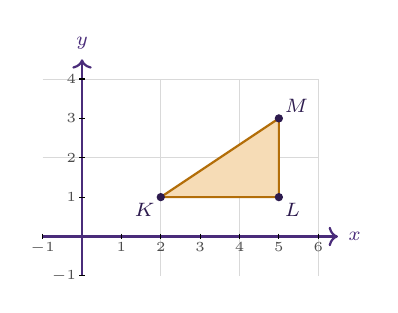
\begin{tikzpicture}[x=0.5cm,y=0.5cm]
\axg{-1}{-1}{6}{4}
\fill[accc!30] (2,1)--(5,1)--(5,3)--cycle;
\draw[accc!80!black,thick] (2,1)--(5,1)--(5,3)--cycle;
\pnt{2}{1}{K}{below left}\pnt{5}{1}{L}{below right}\pnt{5}{3}{M}{above right}
\end{tikzpicture}}}{\pil{$(-3,5)$}{$(3,5)$}{$(5,-3)$}{$(3,-5)$}{$(-3,-5)$}}
\soal{Misalkan $A$ dan $B$ matriks berordo $2\times2$ serta $k$ sebuah skalar. Pilih \emph{semua} pernyataan yang benar.}{\pilk{$(A+B)^{T}=A^{T}+B^{T}$.}{$(AB)^{T}=A^{T}B^{T}$ untuk setiap $A$ dan $B$.}{Jika $AB=O$, maka $A=O$ atau $B=O$.}{Jika $A$ mempunyai invers dan $AB=AC$, maka $B=C$.}{$\det(kA)=k^{2}\det(A)$.}}

\tingkat{Tingkat Sedang}{soal 6 sampai 10}
\soal{Diketahui $A=\begin{bmatrix}4&1\\2&3\end{bmatrix}$. Matriks $A-kI$ tidak mempunyai invers untuk dua nilai $k$. Jumlah kuadrat kedua nilai $k$ tersebut adalah \dots.}{\pil{$7$}{$10$}{$17$}{$21$}{$29$}}
\soal{Dina membeli $2$ gelas kopi dan $3$ potong roti seharga Rp66.000. Eka membeli $3$ gelas kopi dan $1$ potong roti di kafe yang sama seharga Rp57.000. Dengan memakai persamaan matriks, biaya untuk membeli $4$ gelas kopi dan $5$ potong roti adalah \dots.}{\pil{Rp114.000}{Rp120.000}{Rp126.000}{Rp132.000}{Rp138.000}}
\soal{\gbr{Garis $g$ pada gambar ditransformasikan oleh matriks $T=\begin{bmatrix}1&1\\0&1\end{bmatrix}$. Persamaan bayangan garis $g$ adalah \dots.}{%
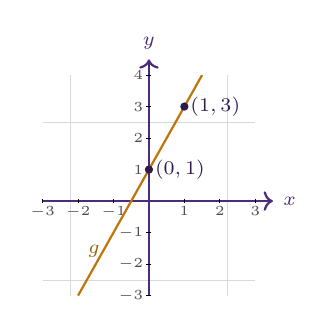
\begin{tikzpicture}[x=0.45cm,y=0.4cm]
\axg{-3}{-3}{3}{4}
\begin{scope}\clip (-3,-3) rectangle (3,4);\draw[thick,accc!85!black] (-2,-3)--(1.5,4);\end{scope}
\pnt{0}{1}{(0,1)}{right}\pnt{1}{3}{(1,3)}{right}
\node[font=\scriptsize,accc!70!black,left,inner sep=1pt] at (-1.3,-1.6) {$g$};
\end{tikzpicture}}}{\pilx{$2x+y+1=0$}{$3x-2y+1=0$}{$2x-3y+1=0$}{$2x-3y-1=0$}{$x-3y+2=0$}}
\soal{\gbr{Sebuah pesan dienkripsi per dua huruf. Setiap huruf diberi kode sesuai tabel, tiap pasangan huruf ditulis sebagai matriks kolom $2\times1$, lalu dikalikan dengan matriks kunci $K=\begin{bmatrix}2&1\\3&2\end{bmatrix}$. Dua pasangan pertama pesan terenkripsi membentuk matriks $\begin{bmatrix}5&7\\8&11\end{bmatrix}$ (kolom pertama untuk pasangan pertama). Pesan aslinya adalah \dots.}{%
\setlength{\tabcolsep}{1.4pt}\renewcommand{\arraystretch}{1.1}\scriptsize
\begin{tabular}{@{}*{13}{c}@{}}
A&B&C&D&E&F&G&H&I&J&K&L&M\\\hline
1&2&3&4&5&6&7&8&9&10&11&12&13\\[3pt]
N&O&P&Q&R&S&T&U&V&W&X&Y&Z\\\hline
14&15&16&17&18&19&20&21&22&23&24&25&26
\end{tabular}}}{\pil{BACA}{BAKA}{BATA}{KACA}{BACU}}
\soal{Diketahui $F=\begin{bmatrix}1&1\\1&0\end{bmatrix}$. Tentukan benar atau salah setiap pernyataan berikut.}{\kat{$F^{4}=\begin{bmatrix}5&3\\3&2\end{bmatrix}$.}{$\det\!\left(F^{10}\right)=-1$.}{$F^{-1}=\begin{bmatrix}0&1\\1&-1\end{bmatrix}$.}{Jumlah semua elemen $F^{6}$ adalah $36$.}}

\tingkat{Tingkat Sulit}{soal 11 sampai 15, setara UTBK}
\soal{Sistem persamaan linear $\begin{bmatrix}a&2\\3&a-1\end{bmatrix}\begin{bmatrix}x\\y\end{bmatrix}=\begin{bmatrix}4\\c\end{bmatrix}$ mempunyai tak hingga banyak penyelesaian. Nilai $ac$ yang mungkin adalah \dots.}{\pil{$-12$}{$-6$}{$6$}{$12$}{$24$}}
\soal{\gbr{Garis $g:y=2x$ pada gambar berperan sebagai cermin. Refleksi terhadap $g$ dinyatakan dengan matriks $R$. Bayangan titik $P(10,5)$ oleh $R$ adalah \dots.}{%
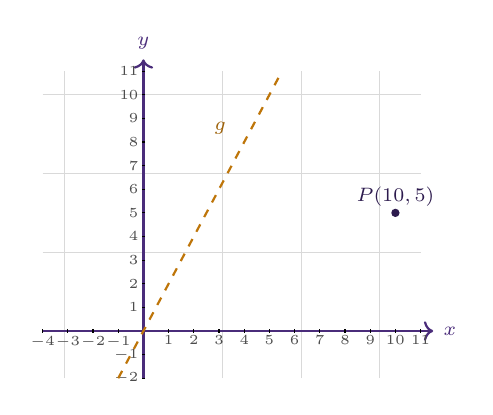
\begin{tikzpicture}[x=0.32cm,y=0.3cm]
\axg{-4}{-2}{11}{11}
\begin{scope}\clip (-4,-2) rectangle (11,11);\draw[dashed,thick,accc!85!black] (-1,-2)--(5.5,11);\end{scope}
\node[font=\scriptsize,accc!70!black,left,inner sep=1pt] at (3.4,8.6) {$g$};
\pnt{10}{5}{P(10,5)}{above}
\end{tikzpicture}}}{\pilx{$(5,10)$}{$(-5,-10)$}{$(10,-5)$}{$(2,11)$}{$(-2,11)$}}
\soal{\gbr{Segitiga $OPQ$ dengan $P(2,1)$ dan $Q(1,3)$ dipetakan oleh sebuah transformasi linear $M$ menjadi segitiga $OP'Q'$ dengan $P'(4,-1)$ dan $Q'(7,2)$ (lihat gambar). Titik yang bayangannya adalah $(5,4)$ oleh $M$ adalah \dots.}{%
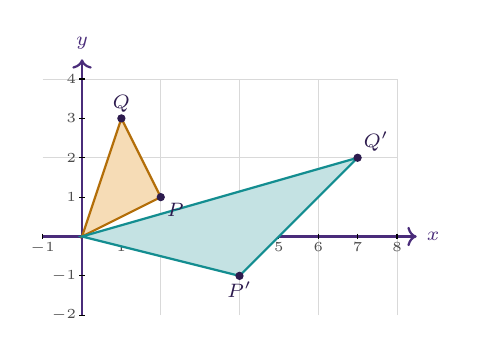
\begin{tikzpicture}[x=0.5cm,y=0.5cm]
\axg{-1}{-2}{8}{4}
\fill[accc!30] (0,0)--(2,1)--(1,3)--cycle;
\fill[warmc!25] (0,0)--(4,-1)--(7,2)--cycle;
\draw[accc!80!black,thick] (0,0)--(2,1)--(1,3)--cycle;
\draw[warmc,thick] (0,0)--(4,-1)--(7,2)--cycle;
\pnt{2}{1}{P}{below right}\pnt{1}{3}{Q}{above}\pnt{4}{-1}{P'}{below}\pnt{7}{2}{Q'}{above right}
\end{tikzpicture}}}{\pil{$(1,-3)$}{$(-1,3)$}{$(3,-1)$}{$(13,-1)$}{$(-3,1)$}}
\soal{\gbr{Perekonomian sederhana memiliki dua sektor, yaitu sektor I (pertanian) dan sektor II (industri). Tabel menunjukkan banyak satuan masukan dari tiap sektor yang diperlukan untuk menghasilkan $1$ satuan keluaran suatu sektor. Permintaan akhir dari luar kedua sektor adalah $30$ satuan untuk sektor I dan $60$ satuan untuk sektor II. Keluaran total $x_1$ dan $x_2$ memenuhi $\mathbf{x}=A\mathbf{x}+\mathbf{d}$ dengan $A$ matriks pada tabel. Pilih \emph{semua} pernyataan yang benar.}{%
\footnotesize\setlength{\tabcolsep}{4pt}\renewcommand{\arraystretch}{1.2}
\begin{tabular}{@{}l|cc@{}}
 & \multicolumn{2}{c}{\textbf{Per 1 satuan keluaran}}\\
\textbf{Masukan dari} & sektor I & sektor II\\\hline
sektor I & $0{,}2$ & $0{,}3$\\
sektor II & $0{,}4$ & $0{,}1$
\end{tabular}}}{\pilk{Keluaran total sektor I adalah $75$ satuan.}{Keluaran total sektor II adalah $90$ satuan.}{Untuk menghasilkan $x_1$, sektor I memakai $30$ satuan keluaran sektor II.}{Sektor I memakai $20$ satuan keluarannya sendiri.}{Jumlah seluruh pemakaian antarsektor adalah $85$ satuan.}}
\soal{Diketahui $A=\begin{bmatrix}2&1\\1&1\end{bmatrix}$, $B=\begin{bmatrix}1&2\\0&1\end{bmatrix}$, dan $C=\begin{bmatrix}5&18\\4&14\end{bmatrix}$. Jika matriks $X$ memenuhi $AXB=C$, jumlah semua elemen $X$ adalah \dots.}{\pil{$7$}{$8$}{$9$}{$10$}{$12$}}

\Needspace{22\baselineskip}\tingkat{Tingkat HOTS}{soal 16 sampai 20, penalaran tingkat tinggi gaya TKA dan UTBK}
\soal{\gbr{Segitiga sama sisi $T_1T_2T_3$ pada gambar mempunyai titik sudut $T_1(1,0)$, $T_2\!\left(-\tfrac12,\tfrac{\sqrt3}{2}\right)$, dan $T_3\!\left(-\tfrac12,-\tfrac{\sqrt3}{2}\right)$. Pilih \emph{semua} matriks yang memetakan segitiga tersebut tepat ke dirinya sendiri, yaitu setiap titik sudut dipetakan ke salah satu titik sudutnya.}{%
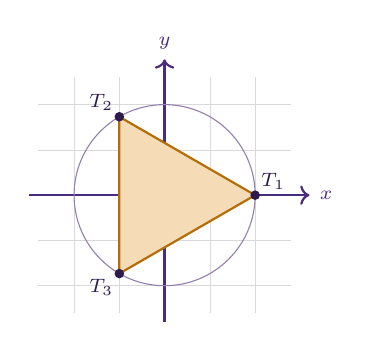
\begin{tikzpicture}[scale=1.15]
\draw[gray!30,very thin] (-1.4,-1.3) grid[step=0.5] (1.4,1.3);
\draw[->,thick,mainc] (-1.5,0)--(1.6,0) node[right,font=\scriptsize]{$x$};
\draw[->,thick,mainc] (0,-1.4)--(0,1.5) node[above,font=\scriptsize]{$y$};
\draw[thin,mainc!60] (0,0) circle (1);
\fill[accc!30] (0:1)--(120:1)--(240:1)--cycle;
\draw[accc!80!black,thick] (0:1)--(120:1)--(240:1)--cycle;
\fill[deepc] (0:1) circle (1.5pt) node[above right,font=\scriptsize,inner sep=2pt]{$T_1$};
\fill[deepc] (120:1) circle (1.5pt) node[above left,font=\scriptsize,inner sep=2pt]{$T_2$};
\fill[deepc] (240:1) circle (1.5pt) node[below left,font=\scriptsize,inner sep=2pt]{$T_3$};
\end{tikzpicture}}}{\pilk{$\sm{-\tfrac12&-\tfrac{\sqrt3}{2}\\\tfrac{\sqrt3}{2}&-\tfrac12}$}{$\sm{\tfrac12&-\tfrac{\sqrt3}{2}\\\tfrac{\sqrt3}{2}&\tfrac12}$}{$\sm{1&0\\0&-1}$}{$\sm{-1&0\\0&1}$}{$\sm{-\tfrac12&\tfrac{\sqrt3}{2}\\-\tfrac{\sqrt3}{2}&-\tfrac12}$}}
\soal{\gbr{Lima peserta duduk di kursi bernomor $1$ sampai $5$. Pada setiap putaran, peserta berpindah kursi sesuai panah pada gambar. Perpindahan ini dinyatakan dengan matriks $P$ berordo $5\times5$: elemen baris ke-$i$ kolom ke-$j$ bernilai $1$ jika peserta di kursi $j$ pindah ke kursi $i$, dan bernilai $0$ untuk lainnya. Nilai $\tr\!\left(P^{2026}\right)$ adalah \dots.}{%
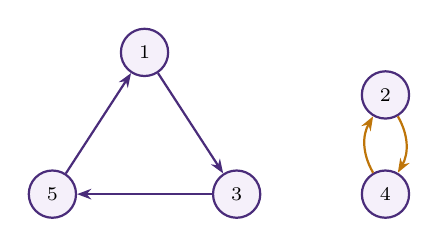
\begin{tikzpicture}[scale=0.9]
\node[nd] (n1) at (0,1.5) {$1$}; \node[nd] (n3) at (1.3,-0.5) {$3$}; \node[nd] (n5) at (-1.3,-0.5) {$5$};
\draw[ar] (n1)--(n3); \draw[ar] (n3)--(n5); \draw[ar] (n5)--(n1);
\node[nd] (n2) at (3.4,0.9) {$2$}; \node[nd] (n4) at (3.4,-0.5) {$4$};
\draw[ar,accc!85!black] (n2) to[bend left=30] (n4); \draw[ar,accc!85!black] (n4) to[bend left=30] (n2);
\end{tikzpicture}}}{\pil{$0$}{$1$}{$2$}{$3$}{$5$}}
\soal{Banyak matriks berordo $2\times2$ yang setiap elemennya salah satu dari $-1$, $0$, atau $1$ dan mempunyai invers adalah \dots.}{\pil{$48$}{$54$}{$64$}{$72$}{$81$}}

\Needspace{16\baselineskip}\par\vspace{0.75em}
\begin{tcolorbox}[colback=softbg,colframe=accc,boxrule=0.8pt,arc=3pt,left=7pt,right=7pt,top=4pt,bottom=4pt,title={\bfseries Stimulus untuk soal 19 dan 20},coltitle=white,fonttitle=\small]
\gbr{Sebuah aplikasi animasi memiliki tiga tombol. Tombol \textbf{S} menggeser objek mendatar dengan matriks $S=\sm{1&1\\0&1}$; tombol \textbf{D} meregangkan objek ke arah sumbu-$y$ dengan matriks $D=\sm{1&0\\0&2}$; tombol \textbf{F} mencerminkan objek terhadap sumbu-$y$ dengan matriks $F=\sm{-1&0\\0&1}$. Satu \emph{paket} berarti menekan S, D, F berturut-turut. Logo berbentuk segitiga $ABC$ dengan $A(1,1)$, $B(3,1)$, dan $C(1,3)$ (lihat gambar) diubah memakai paket tersebut.}{%
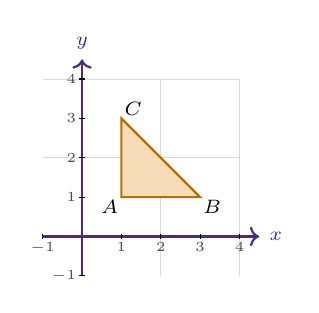
\begin{tikzpicture}[x=0.5cm,y=0.5cm]
\axg{-1}{-1}{4}{4}
\fill[accc!30] (1,1)--(3,1)--(1,3)--cycle;
\draw[accc!80!black,thick] (1,1)--(3,1)--(1,3)--cycle;
\node[font=\scriptsize,below left,inner sep=1pt] at (1,1) {$A$};
\node[font=\scriptsize,below right,inner sep=1pt] at (3,1) {$B$};
\node[font=\scriptsize,above right,inner sep=1pt] at (1,3) {$C$};
\end{tikzpicture}}
\end{tcolorbox}
\soal{Jika paket ditekan dua kali berturut-turut (enam tombol), koordinat bayangan akhir titik $C$ adalah \dots.}{\pil{$(0,4)$}{$(2,4)$}{$(-2,6)$}{$(-4,6)$}{$(-2,12)$}}
\soal{Tentukan benar atau salah setiap pernyataan berikut.}{\kat{Luas bayangan segitiga $ABC$ setelah \emph{satu} paket adalah $4$ satuan luas.}{Pada bayangan setelah satu paket, urutan titik $A'\to B'\to C'$ searah jarum jam, sedangkan urutan $A\to B\to C$ berlawanan arah jarum jam.}{Terdapat titik tak nol yang posisinya tidak berubah setelah satu paket.}{Setelah \emph{tiga} paket, luas bayangan sama dengan $8$ kali luas segitiga semula.}}

% =====================================================================
\Needspace{16\baselineskip}
\bagian{B. Isian Singkat}{5 soal $\times$ 4 poin = 20 poin. Tuliskan hanya jawaban akhir.}

\tingkat{Tingkat Sedang}{soal 1 dan 2}
\soal{Matriks $A=\begin{bmatrix}x&2&1\\0&x-1&3\\0&0&2\end{bmatrix}$ mempunyai determinan $12$. Jumlah kuadrat semua nilai $x$ yang memenuhi adalah \dots.}{\jwb}
\soal{Titik $P(a,b)$ didilatasi berpusat di $O(0,0)$ dengan faktor $3$, kemudian bayangannya dicerminkan terhadap garis $y=-x$ sehingga menjadi titik $(6,-9)$. Nilai $a-b$ adalah \dots.}{\jwb}

\tingkat{Tingkat Sulit}{soal 3 sampai 5}
\soal{\gbr{Matriks $M$ berordo $4\times4$ mempunyai elemen $m_{ij}=|i-j|$ (lihat gambar; elemen diagonal utama bernilai $0$). Nilai $\det(M)$ adalah \dots.}{%
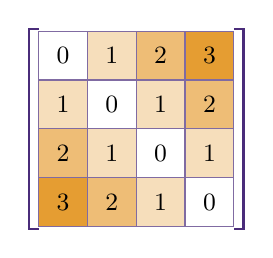
\begin{tikzpicture}[scale=0.62]
\foreach \r in {0,...,3}{\foreach \c in {0,...,3}{%
  \pgfmathtruncatemacro{\v}{abs(\r-\c)}\pgfmathtruncatemacro{\p}{\v*28}
  \node[draw=mainc!70,fill=accc!\p,minimum size=0.62cm,inner sep=0pt,font=\small] at (\c,-\r) {$\v$};}}
\draw[mainc,thick] (-0.5,0.55) -- (-0.7,0.55) -- (-0.7,-3.55) -- (-0.5,-3.55);
\draw[mainc,thick] (3.5,0.55) -- (3.7,0.55) -- (3.7,-3.55) -- (3.5,-3.55);
\end{tikzpicture}}}{\jwb}
\soal{Matriks $A$ berordo $2\times2$ memenuhi $\tr(A)=4$ dan $\tr(A^{2})=10$. Nilai $\tr(A^{3})$ adalah \dots.}{\jwb}
\soal{\gbr{Lengan robot terdiri atas dua ruas. Ruas pertama $OJ$ panjangnya $6$ dm dan ruas kedua $JE$ panjangnya $4$ dm. Mula-mula kedua ruas lurus sepanjang sumbu-$x$ positif (garis putus-putus pada gambar). Sendi $O$ memutar seluruh lengan sebesar $60^\circ$ berlawanan arah jarum jam, kemudian sendi $J$ memutar ruas kedua sebesar $120^\circ$ searah jarum jam terhadap arah ruas pertama. Jarak ujung $E$ ke titik $O$ adalah \dots\ dm.}{%
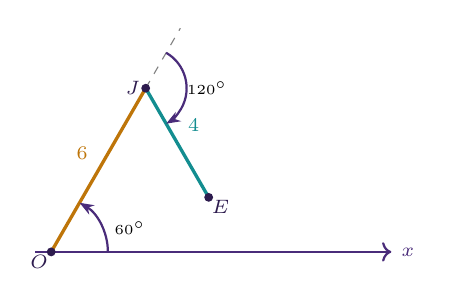
\begin{tikzpicture}[x=0.4cm,y=0.4cm]
\draw[dashed,gray!70,thick] (0,0)--(10,0);
\draw[->,thick,mainc] (-0.5,0)--(10.8,0) node[right,font=\scriptsize]{$x$};
\coordinate (O) at (0,0); \coordinate (J) at (3,5.196); \coordinate (E) at (5,1.732);
\draw[dashed,gray] (J)--($(J)+(60:2.2)$);
\draw[accc!85!black,very thick] (O)--(J) node[midway,above left,font=\scriptsize]{$6$};
\draw[warmc,very thick] (J)--(E) node[midway,above right,font=\scriptsize]{$4$};
\draw[ar] (1.8,0) arc[start angle=0,end angle=60,radius=1.8];
\node[font=\tiny] at (2.5,0.75) {$60^\circ$};
\draw[ar] ($(J)+(60:1.3)$) arc[start angle=60,end angle=-60,radius=1.3];
\node[font=\tiny] at ($(J)+(1.95,0)$) {$120^\circ$};
\fill[deepc] (O) circle (1.6pt) node[below left,font=\scriptsize,inner sep=1pt]{$O$};
\fill[deepc] (J) circle (1.6pt) node[left,font=\scriptsize,inner sep=2pt]{$J$};
\fill[deepc] (E) circle (1.6pt) node[below right,font=\scriptsize,inner sep=1pt]{$E$};
\end{tikzpicture}}}{\jwb}

% =====================================================================
\Needspace{16\baselineskip}
\bagian{C. Uraian}{5 soal $\times$ 8 poin = 40 poin. Tuliskan langkah penyelesaian dengan lengkap.}

\tingkat{Tingkat Sedang}{soal 1 dan 2}
\soal{\gbr{Dua gerai kue, $G_1$ dan $G_2$, menjual brownies, bolu, dan donat. Banyak kue terjual dalam sehari ditulis sebagai matriks $P$ (baris: gerai; kolom: brownies, bolu, donat). Biaya produksi per kue (dalam ribuan rupiah) ditulis sebagai matriks $B$ (baris: jenis kue; kolom: bahan, tenaga kerja). Harga jual per kue (ribuan rupiah) ditulis sebagai matriks kolom $H$ (lihat tabel).\par\smallskip
(a) Hitung $PB$ dan jelaskan arti setiap elemennya.\par
(b) Dengan perkalian matriks, tentukan pendapatan dan laba tiap gerai (laba = pendapatan $-$ total biaya).\par
(c) Biaya bahan naik $10\%$ sedangkan biaya tenaga kerja tetap. Tulis matriks biaya baru $B'=BD$ dengan $D$ matriks diagonal berordo $2\times2$, lalu hitung laba baru tiap gerai.\par
(d) Hitung penurunan laba total kedua gerai, lalu tunjukkan bahwa nilainya sama dengan $10\%$ dari total biaya bahan seluruh gerai sebelum kenaikan.}{%
\small\renewcommand{\arraystretch}{1.15}
\begin{tabular}{@{}l|ccc@{}}
$P$ & Brw & Blu & Dnt\\\hline
$G_1$ & $20$ & $10$ & $30$\\
$G_2$ & $15$ & $25$ & $10$
\end{tabular}\par\medskip
\begin{tabular}{@{}l|cc@{}}
$B$ & Bahan & Tenaga\\\hline
Brownies & $3$ & $1$\\
Bolu & $2$ & $1$\\
Donat & $1$ & $0{,}5$
\end{tabular}\par\medskip
\begin{tabular}{@{}l|c@{}}
$H$ & Harga\\\hline
Brownies & $9$\\
Bolu & $6$\\
Donat & $4$
\end{tabular}}}{\poin{8}}
\soal{\gbr{Koordinat $(x,y)$ pada peta lama diubah menjadi koordinat $(x',y')$ pada peta baru oleh $\begin{bmatrix}x'\\y'\end{bmatrix}=M\begin{bmatrix}x\\y\end{bmatrix}$ dengan $M=\begin{bmatrix}1&-1\\1&1\end{bmatrix}$. Mercusuar berada di $P(3,1)$ dan dermaga di $Q(1,3)$ pada peta lama (lihat gambar).\par\smallskip
(a) Tentukan koordinat $P'$ dan $Q'$ pada peta baru.\par
(b) Tunjukkan bahwa $M=\sqrt2\,R(45^\circ)$, lalu jelaskan arti geometris transformasi $M$.\par
(c) Buktikan bahwa $P'Q'=\sqrt2\cdot PQ$ dan bahwa $\angle POP'=45^\circ$ dengan hasil kali titik dua vektor.\par
(d) Sebuah kapal berada di $K'(6,2)$ pada peta baru. Tentukan posisinya pada peta lama dengan $M^{-1}$.}{%
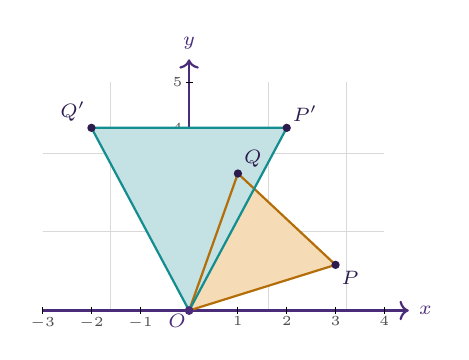
\begin{tikzpicture}[x=0.62cm,y=0.58cm]
\axg{-3}{0}{4}{5}
\fill[accc!30] (0,0)--(3,1)--(1,3)--cycle;
\fill[warmc!25] (0,0)--(2,4)--(-2,4)--cycle;
\draw[accc!80!black,thick] (0,0)--(3,1)--(1,3)--cycle;
\draw[warmc,thick] (0,0)--(2,4)--(-2,4)--cycle;
\pnt{3}{1}{P}{below right}\pnt{1}{3}{Q}{above right}\pnt{2}{4}{P'}{above right}\pnt{-2}{4}{Q'}{above left}
\fill[mainc] (0,0) circle (1.6pt) node[below left,font=\scriptsize,inner sep=1pt]{$O$};
\end{tikzpicture}}}{\poin{8}}

\Needspace{22\baselineskip}\tingkat{Tingkat Sulit}{soal 3 dan 4}
\soal{\gbr{Pada sebuah kawasan, empat persimpangan $A$, $B$, $C$, dan $D$ dihubungkan jalan satu arah seperti pada gambar. Banyak kendaraan per jam pada ruas $A\to B$, $B\to C$, $C\to D$, dan $D\to A$ berturut-turut $x_1$, $x_2$, $x_3$, dan $x_4$. Banyak kendaraan yang masuk dari dan keluar ke jalan lain tertulis pada gambar. Di setiap persimpangan, banyak kendaraan masuk sama dengan banyak kendaraan keluar.\par\smallskip
(a) Susun sistem persamaan linear untuk $x_1,\dots,x_4$ dan tulis dalam bentuk $M\mathbf{x}=\mathbf{b}$.\par
(b) Dengan operasi baris elementer, ubah matriks augmented ke bentuk eselon baris tereduksi. Tunjukkan bahwa sistem mempunyai tak hingga banyak solusi, lalu nyatakan solusi umumnya dengan parameter $s=x_4$.\par
(c) Setiap ruas hanya dapat dilalui paling banyak $400$ kendaraan per jam dan tidak boleh bernilai negatif. Tentukan batas nilai $s$.\par
(d) Mungkinkah ruas $C\to D$ ditutup ($x_3=0$)? Jelaskan. Kemudian tentukan jumlah arus $x_1+x_2+x_3+x_4$ terkecil yang mungkin.}{%
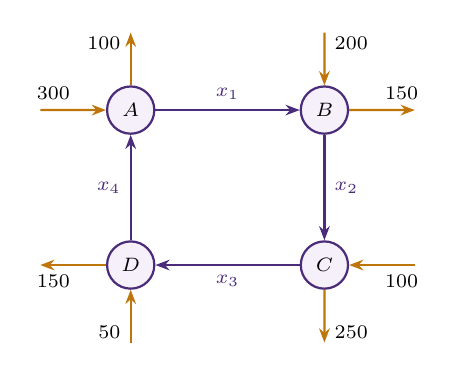
\begin{tikzpicture}[scale=0.82]
\node[nd] (A) at (0,2.4) {$A$}; \node[nd] (B) at (3,2.4) {$B$};
\node[nd] (C) at (3,0) {$C$}; \node[nd] (D) at (0,0) {$D$};
\draw[ar] (A)--(B) node[midway,above,font=\scriptsize]{$x_1$};
\draw[ar] (B)--(C) node[midway,right,font=\scriptsize]{$x_2$};
\draw[ar] (C)--(D) node[midway,below,font=\scriptsize]{$x_3$};
\draw[ar] (D)--(A) node[midway,left,font=\scriptsize]{$x_4$};
\draw[ar,accc!85!black] (-1.4,2.4)--(A) node[pos=0.2,above,font=\scriptsize,text=black]{$300$};
\draw[ar,accc!85!black] (A)--(0,3.6) node[pos=0.8,left,font=\scriptsize,text=black]{$100$};
\draw[ar,accc!85!black] (3,3.6)--(B) node[pos=0.2,right,font=\scriptsize,text=black]{$200$};
\draw[ar,accc!85!black] (B)--(4.4,2.4) node[pos=0.8,above,font=\scriptsize,text=black]{$150$};
\draw[ar,accc!85!black] (4.4,0)--(C) node[pos=0.2,below,font=\scriptsize,text=black]{$100$};
\draw[ar,accc!85!black] (C)--(3,-1.2) node[pos=0.8,right,font=\scriptsize,text=black]{$250$};
\draw[ar,accc!85!black] (0,-1.2)--(D) node[pos=0.2,left,font=\scriptsize,text=black]{$50$};
\draw[ar,accc!85!black] (D)--(-1.4,0) node[pos=0.8,below,font=\scriptsize,text=black]{$150$};
\end{tikzpicture}}}{\poin{8}}
\soal{\gbr{Lingkaran $L:x^{2}+y^{2}=1$ ditransformasikan oleh matriks $M=\begin{bmatrix}1&1\\0&2\end{bmatrix}$ menjadi kurva $L'$ (lihat gambar).\par\smallskip
(a) Tentukan bayangan titik $(1,0)$, $(0,1)$, $(-1,0)$, dan $(0,-1)$ pada lingkaran $L$.\par
(b) Tentukan persamaan kurva $L'$ dengan memakai $M^{-1}$, lalu periksa keempat titik pada (a) memenuhi persamaan tersebut.\par
(c) Hitung luas daerah yang dibatasi $L'$ dan jelaskan alasannya memakai determinan.\par
(d) Tentukan koordinat titik pada $L'$ yang absisnya terbesar, lalu tentukan titik pada $L$ yang dipetakan ke titik tersebut.}{%
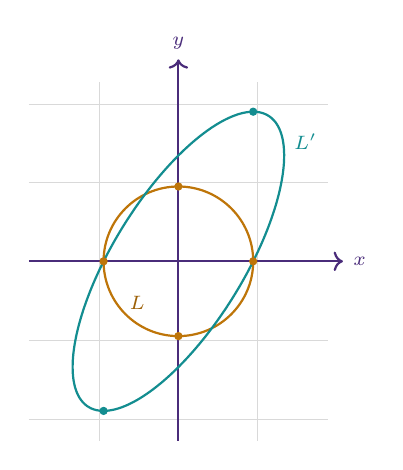
\begin{tikzpicture}[x=0.95cm,y=0.95cm]
\draw[gray!30,very thin] (-2,-2.4) grid (2,2.4);
\draw[->,thick,mainc] (-2,0)--(2.2,0) node[right,font=\scriptsize]{$x$};
\draw[->,thick,mainc] (0,-2.4)--(0,2.7) node[above,font=\scriptsize]{$y$};
\draw[accc!85!black,thick] (0,0) circle (1);
\draw[warmc,thick,smooth,samples=80,domain=0:360] plot ({cos(\x)+sin(\x)},{2*sin(\x)});
\fill[accc!85!black] (1,0) circle (1.5pt) (0,1) circle (1.5pt) (-1,0) circle (1.5pt) (0,-1) circle (1.5pt);
\fill[warmc] (1,2) circle (1.5pt) (-1,-2) circle (1.5pt);
\node[font=\scriptsize,accc!70!black] at (-0.55,-0.55) {$L$};
\node[font=\scriptsize,warmc] at (1.7,1.6) {$L'$};
\end{tikzpicture}}}{\poin{8}}

\Needspace{24\baselineskip}\tingkat{Tingkat HOTS}{soal 5}
\soal{\gbr{Dua cermin datar tegak lurus bidang gambar dan berpotongan di titik asal $O$. Cermin $m_1$ berimpit dengan sumbu-$x$, dan cermin $m_2$ membentuk sudut $30^\circ$ terhadap sumbu-$x$ positif. Refleksi terhadap garis melalui $O$ yang membentuk sudut $\theta$ dengan sumbu-$x$ dilambangkan $M_\theta$. Titik $Q(0,2)$ dipantulkan oleh $m_1$ lalu oleh $m_2$ (lihat gambar).\par\smallskip
(a) Dengan menentukan bayangan vektor basis $\sm{1\\0}$ dan $\sm{0\\1}$, turunkan bahwa $M_\theta=\sm{\cos2\theta&\sin2\theta\\\sin2\theta&-\cos2\theta}$.\par
(b) Hitung $M_0$, $M_{30^\circ}$, $M_{30^\circ}M_0$, dan $M_0M_{30^\circ}$. Tunjukkan bahwa kedua hasil kali berupa rotasi, lalu tentukan besar dan arahnya. Tentukan pula bayangan akhir $Q$.\par
(c) Buktikan secara umum bahwa $M_\beta M_\alpha=\sm{\cos2(\beta-\alpha)&-\sin2(\beta-\alpha)\\\sin2(\beta-\alpha)&\cos2(\beta-\alpha)}$.\par
(d) Sekarang kedua cermin membentuk sudut $20^\circ$ (cermin $m_1$ pada sumbu-$x$ dan $m_2$ pada $20^\circ$). Sebuah titik dipantulkan bergantian oleh $m_1$, $m_2$, $m_1$, $m_2$, dan seterusnya. Tentukan banyak pasangan pantulan paling sedikit sampai titik tersebut kembali ke posisi semula, lalu tentukan banyak pantulan seluruhnya. Mengapa banyak pantulan harus genap?}{%
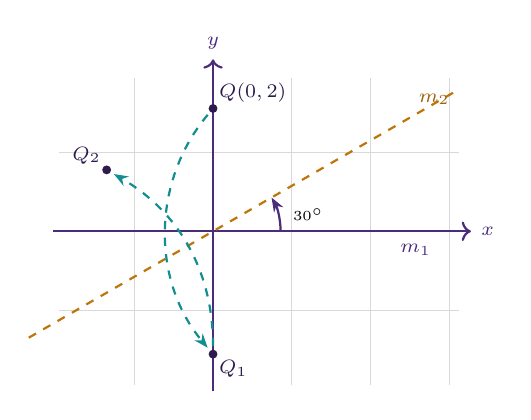
\begin{tikzpicture}[x=0.78cm,y=0.78cm]
\draw[gray!30,very thin] (-2.5,-2.5) grid (4,2.5);
\draw[->,thick,mainc] (-2.6,0)--(4.2,0) node[right,font=\scriptsize]{$x$};
\draw[->,thick,mainc] (0,-2.6)--(0,2.8) node[above,font=\scriptsize]{$y$};
\draw[dashed,thick,accc!85!black] (-3,-1.732)--(4,2.309);
\node[font=\scriptsize,accc!70!black,above] at (3.6,1.9) {$m_2$};
\node[font=\scriptsize,mainc,below] at (3.3,-0.05) {$m_1$};
\draw[ar] (1.1,0) arc[start angle=0,end angle=30,radius=1.1];
\node[font=\tiny] at (1.55,0.27) {$30^\circ$};
\fill[deepc] (0,2) circle (1.6pt) node[above right,font=\scriptsize,inner sep=2pt]{$Q(0,2)$};
\fill[deepc] (0,-2) circle (1.6pt) node[below right,font=\scriptsize,inner sep=2pt]{$Q_1$};
\fill[deepc] (-1.732,1) circle (1.6pt) node[above left,font=\scriptsize,inner sep=2pt]{$Q_2$};
\draw[ar,warmc,dashed,shorten >=3pt,shorten <=3pt] (0,2) to[bend right=40] (0,-2);
\draw[ar,warmc,dashed,shorten >=3pt,shorten <=3pt] (0,-2) to[bend right=30] (-1.732,1);
\end{tikzpicture}}}{\poin{8}}

% =====================================================================
\newpage
\bagian{Kunci Jawaban dan Pembahasan Singkat}{Untuk guru dan pembahasan mandiri}
\par\vspace{0.6em}{\bfseries\color{mainc}Kunci Pilihan Ganda}\par\vspace{0.3em}
\small
\begin{tabularx}{\linewidth}{@{}*{10}{>{\centering\arraybackslash}X}@{}}\hline \textbf{1} & \textbf{2} & \textbf{3} & \textbf{4} & \textbf{5} & \textbf{6} & \textbf{7} & \textbf{8} & \textbf{9} & \textbf{10}\\ \hline B & C & A & D & {\scriptsize A,D,E} & E & B & C & A & {\scriptsize B,S,B,S}\\ \hline\end{tabularx}\\[6pt]
\begin{tabularx}{\linewidth}{@{}*{10}{>{\centering\arraybackslash}X}@{}}\hline \textbf{11} & \textbf{12} & \textbf{13} & \textbf{14} & \textbf{15} & \textbf{16} & \textbf{17} & \textbf{18} & \textbf{19} & \textbf{20}\\ \hline D & E & B & {\scriptsize A,C,E} & D & {\scriptsize A,C,E} & C & A & E & {\scriptsize B,B,S,B}\\ \hline\end{tabularx}
\par\vspace{0.8em}{\bfseries\color{mainc}\normalsize Pembahasan Pilihan Ganda}\par\vspace{0.2em}
\small\begin{enumerate}[leftmargin=2em,itemsep=2pt,topsep=2pt]
\item[\textbf{1.}] \textbf{(B)} $A$ berordo $2\times3$ sehingga $B=A^T$ berordo $3\times2$ dengan $b_{ij}=a_{ji}$. Maka $b_{31}=a_{13}=4$ dan $b_{22}=a_{22}=3$, jumlahnya $7$.
\item[\textbf{2.}] \textbf{(C)} Nilai akhir $=S\mathbf{w}$ dengan $\mathbf{w}=(0{,}3;\,0{,}3;\,0{,}4)^T$. Rina: $24+21+36=81$; Budi: $18+27+30=75$; Citra: $25{,}5+24+28=77{,}5$. Selisih tertinggi dan terendah $=81-75=6$. (Jebakan B: memakai rata-rata biasa, tanpa bobot, memberi $80$ dan $75$ sehingga selisihnya $5$.)
\item[\textbf{3.}] \textbf{(A)} Tidak mempunyai invers berarti $\det=0$: $k(k+1)-12=k^2+k-12=(k+4)(k-3)=0$, sehingga $k=-4$ atau $k=3$. Nilai positifnya $3$.
\item[\textbf{4.}] \textbf{(D)} $\begin{bmatrix}0&1\\-1&0\end{bmatrix}\begin{bmatrix}5\\3\end{bmatrix}=\begin{bmatrix}3\\-5\end{bmatrix}$, yaitu $(x,y)\mapsto(y,-x)$. (Jebakan A: memakai rotasi berlawanan arah jarum jam, $(x,y)\mapsto(-y,x)$.)
\item[\textbf{5.}] \textbf{(A, D, E)} A benar: transpose menjumlahkan secara linear. B salah: yang benar $(AB)^T=B^TA^T$. C salah: ada matriks tak nol $A,B$ dengan $AB=O$, misalnya $\sm{1&0\\0&0}\sm{0&0\\0&1}$. D benar: kalikan kedua ruas dengan $A^{-1}$ dari kiri. E benar: $2\times2$ dan setiap baris dikali $k$, sehingga determinan dikali $k\cdot k$.
\item[\textbf{6.}] \textbf{(E)} $\det(A-kI)=(4-k)(3-k)-2=k^2-7k+10=0$, sehingga $k=2$ atau $k=5$. Jumlah kuadrat $=2^2+5^2=29$, atau $(k_1+k_2)^2-2k_1k_2=49-20=29$. (Jebakan A: $7$ adalah jumlah akar; B: $10$ hasil kali akar.)
\item[\textbf{7.}] \textbf{(B)} Misalkan harga kopi $c$ dan roti $r$ (ribuan rupiah). $\begin{bmatrix}2&3\\3&1\end{bmatrix}\begin{bmatrix}c\\r\end{bmatrix}=\begin{bmatrix}66\\57\end{bmatrix}$ dengan $\det=-7$. $\begin{bmatrix}c\\r\end{bmatrix}=\frac{1}{-7}\begin{bmatrix}1&-3\\-3&2\end{bmatrix}\begin{bmatrix}66\\57\end{bmatrix}=\begin{bmatrix}15\\12\end{bmatrix}$. Biaya $4c+5r=60+60=120$, yaitu Rp120.000.
\item[\textbf{8.}] \textbf{(C)} Titik $(x,y)$ menjadi $(x',y')=(x+y,\,y)$, sehingga $y=y'$ dan $x=x'-y'$. Substitusi ke $y=2x+1$: $y'=2(x'-y')+1\Rightarrow3y'=2x'+1$, yaitu $2x-3y+1=0$. Cek: $(0,1)\mapsto(1,1)$ dan $(1,3)\mapsto(4,3)$, keduanya memenuhi. (Jebakan A: mensubstitusi $(x'+y',y')$ ke persamaan asal, yaitu memakai $T$ dan bukan $T^{-1}$.)
\item[\textbf{9.}] \textbf{(A)} $\det K=1$, sehingga $K^{-1}=\begin{bmatrix}2&-1\\-3&2\end{bmatrix}$. Pesan $=K^{-1}\begin{bmatrix}5&7\\8&11\end{bmatrix}=\begin{bmatrix}2&3\\1&1\end{bmatrix}$. Kolom pertama $(2,1)$ adalah B, A dan kolom kedua $(3,1)$ adalah C, A, jadi pesannya BACA. Cek: $K\begin{bmatrix}2\\1\end{bmatrix}=\begin{bmatrix}5\\8\end{bmatrix}$.
\item[\textbf{10.}] \textbf{(B, S, B, S)} $F^2=\sm{2&1\\1&1}$, $F^3=\sm{3&2\\2&1}$, $F^4=\sm{5&3\\3&2}$ (elemennya bilangan Fibonacci): (1) \emph{benar}. $\det F=-1$ sehingga $\det F^{10}=(-1)^{10}=1$: (2) \emph{salah}. $F^{-1}=\frac{1}{-1}\sm{0&-1\\-1&1}=\sm{0&1\\1&-1}$: (3) \emph{benar}. $F^6=\sm{13&8\\8&5}$ berjumlah $34$, bukan $36$: (4) \emph{salah}.
\item[\textbf{11.}] \textbf{(D)} Tak hingga solusi mensyaratkan $\det=0$: $a(a-1)-6=0$, sehingga $a=3$ atau $a=-2$. Untuk $a=3$: baris $(3,2\mid4)$ dan $(3,2\mid c)$ sama jika $c=4$. Untuk $a=-2$: baris $(-2,2\mid4)$ dan $(3,-3\mid c)$; baris kedua $=-\tfrac32\times$ baris pertama jika $c=-6$. Kedua kasus memberi $ac=12$.
\item[\textbf{12.}] \textbf{(E)} Garis $y=2x$ membentuk sudut $\theta$ dengan $\tan\theta=2$. $\cos2\theta=\frac{1-4}{1+4}=-\frac35$ dan $\sin2\theta=\frac{2\cdot2}{1+4}=\frac45$. $R=\begin{bmatrix}\cos2\theta&\sin2\theta\\\sin2\theta&-\cos2\theta\end{bmatrix}=\begin{bmatrix}-\frac35&\frac45\\\frac45&\frac35\end{bmatrix}$. $R\begin{bmatrix}10\\5\end{bmatrix}=\begin{bmatrix}-6+4\\8+3\end{bmatrix}=\begin{bmatrix}-2\\11\end{bmatrix}$. Cek: titik tengah $(4,8)$ terletak pada $g$, dan gradien $PP'=\frac{6}{-12}=-\frac12$ tegak lurus gradien $g$. (Jebakan D: salah tanda pada komponen pertama.)
\item[\textbf{13.}] \textbf{(B)} Dari $M\begin{bmatrix}2&1\\1&3\end{bmatrix}=\begin{bmatrix}4&7\\-1&2\end{bmatrix}$ dan $\det\begin{bmatrix}2&1\\1&3\end{bmatrix}=5$: $M=\begin{bmatrix}4&7\\-1&2\end{bmatrix}\cdot\frac15\begin{bmatrix}3&-1\\-1&2\end{bmatrix}=\begin{bmatrix}1&2\\-1&1\end{bmatrix}$. $\det M=3$ dan $M^{-1}=\frac13\begin{bmatrix}1&-2\\1&1\end{bmatrix}$. Titik asal $=M^{-1}\begin{bmatrix}5\\4\end{bmatrix}=\frac13\begin{bmatrix}-3\\9\end{bmatrix}=\begin{bmatrix}-1\\3\end{bmatrix}$. Cek: $M(-1,3)=(5,4)$. (Jebakan D: $M(5,4)=(13,-1)$, yaitu mencari bayangan, bukan prapeta.)
\item[\textbf{14.}] \textbf{(A, C, E)} $(I-A)\mathbf{x}=\mathbf{d}$ dengan $I-A=\begin{bmatrix}0{,}8&-0{,}3\\-0{,}4&0{,}9\end{bmatrix}$, $\det=0{,}72-0{,}12=0{,}6$. $\mathbf{x}=\frac{1}{0{,}6}\begin{bmatrix}0{,}9&0{,}3\\0{,}4&0{,}8\end{bmatrix}\begin{bmatrix}30\\60\end{bmatrix}=\frac{1}{0{,}6}\begin{bmatrix}45\\60\end{bmatrix}=\begin{bmatrix}75\\100\end{bmatrix}$. A benar; B salah ($x_2=100$). C benar: $0{,}4\times75=30$. D salah: $0{,}2\times75=15$. E benar: pemakaian antarsektor $=(15+30)+(30+10)=85$, dan cocok dengan $175-90=85$ (total keluaran dikurangi permintaan akhir).
\item[\textbf{15.}] \textbf{(D)} $X=A^{-1}CB^{-1}$ dengan $A^{-1}=\begin{bmatrix}1&-1\\-1&2\end{bmatrix}$ dan $B^{-1}=\begin{bmatrix}1&-2\\0&1\end{bmatrix}$. $A^{-1}C=\begin{bmatrix}1&4\\3&10\end{bmatrix}$, lalu $X=\begin{bmatrix}1&2\\3&4\end{bmatrix}$. Jumlah elemen $=10$.
\item[\textbf{16.}] \textbf{(A, C, E)} Matriks memetakan segitiga ke dirinya jika himpunan $\{T_1,T_2,T_3\}$ dipetakan ke dirinya sendiri. A: rotasi $120^\circ$, $T_1\to T_2\to T_3\to T_1$ (benar). B: rotasi $60^\circ$ memetakan $T_1$ ke $\left(\frac12,\frac{\sqrt3}{2}\right)$ yang bukan titik sudut (salah). C: refleksi terhadap sumbu-$x$ menukar $T_2$ dan $T_3$, $T_1$ tetap (benar). D: refleksi terhadap sumbu-$y$ memetakan $T_1$ ke $(-1,0)$ (salah). E: rotasi $240^\circ$, $T_1\to T_3\to T_2\to T_1$ (benar).
\item[\textbf{17.}] \textbf{(C)} Kursi $1\to3\to5\to1$ membentuk siklus panjang $3$, dan kursi $2\leftrightarrow4$ saling bertukar (siklus panjang $2$). Elemen diagonal $P^{n}$ bernilai $1$ hanya untuk kursi yang kembali ke tempatnya setelah $n$ putaran, sehingga $\tr(P^{n})$ adalah banyak kursi yang kembali. $2026=3\cdot675+1$ sehingga kursi $1,3,5$ belum kembali (tiap peserta maju satu langkah siklus). $2026$ genap sehingga kursi $2$ dan $4$ kembali. Jadi $\tr(P^{2026})=2$. (Jebakan E: menganggap $P^{2026}=I$; $P^{n}=I$ pertama kali saat $n=\mathrm{KPK}(3,2)=6$.)
\item[\textbf{18.}] \textbf{(A)} Ada $3^4=81$ matriks. Matriks tak punya invers jika $ad=bc$. Hasil kali dua elemen $\{-1,0,1\}$: bernilai $0$ pada $5$ dari $9$ pasangan, bernilai $1$ pada $2$ pasangan, dan bernilai $-1$ pada $2$ pasangan. Banyak $(a,d,b,c)$ dengan $ad=bc$ adalah $5\cdot5+2\cdot2+2\cdot2=33$. Yang mempunyai invers: $81-33=48$.
\item[\textbf{19.}] \textbf{(E)} Satu paket: $T=FDS$ (S dikerjakan lebih dulu). $DS=\begin{bmatrix}1&1\\0&2\end{bmatrix}$ dan $T=F(DS)=\begin{bmatrix}-1&-1\\0&2\end{bmatrix}$. $T(1,3)=(-4,6)$ (jebakan D: baru satu paket), lalu $T(-4,6)=(4-6,\,12)=(-2,12)$. Cek dengan $T^2=\begin{bmatrix}1&-1\\0&4\end{bmatrix}$: $T^2\begin{bmatrix}1\\3\end{bmatrix}=\begin{bmatrix}-2\\12\end{bmatrix}$.
\item[\textbf{20.}] \textbf{(B, B, S, B)} $\det T=-2$ dan luas $\triangle ABC=\frac12\cdot2\cdot2=2$. (1) Luas setelah satu paket $=|\det T|\cdot2=4$: \emph{benar}. (2) $A'(-2,2)$, $B'(-4,2)$, $C'(-4,6)$ berputar searah jarum jam, sedangkan $\det T<0$ membalik orientasi: \emph{benar}. (3) Titik tetap memenuhi $(T-I)\mathbf{v}=\mathbf{0}$ dengan $\det(T-I)=\det\begin{bmatrix}-2&-1\\0&1\end{bmatrix}=-2\ne0$, sehingga hanya $\mathbf{v}=\mathbf{0}$ (titik asal): \emph{salah}. (4) Luas setelah tiga paket $=|\det T|^{3}\cdot$ luas semula $=8\times$ luas semula: \emph{benar}.
\end{enumerate}
\par\Needspace{6\baselineskip}\vspace{0.6em}{\bfseries\color{mainc}\normalsize Pembahasan Isian Singkat}\par\vspace{0.2em}
\small\begin{enumerate}[leftmargin=2em,itemsep=2pt,topsep=2pt]
\item[\textbf{1.}] \textbf{Jawaban: $13$.} Matriks segitiga atas: determinan $=$ hasil kali elemen diagonal $=x(x-1)\cdot2=12$, sehingga $x^2-x-6=0$ dan $x=3$ atau $x=-2$. Jumlah kuadrat $=9+4=13$.
\item[\textbf{2.}] \textbf{Jawaban: $5$.} Dilatasi: $\begin{bmatrix}3&0\\0&3\end{bmatrix}$. Refleksi terhadap $y=-x$: $\begin{bmatrix}0&-1\\-1&0\end{bmatrix}$. Matriks komposisi $\begin{bmatrix}0&-3\\-3&0\end{bmatrix}$, sehingga $(-3b,\,-3a)=(6,-9)$. Maka $b=-2$, $a=3$, dan $a-b=5$.
\item[\textbf{3.}] \textbf{Jawaban: $-12$.} Lakukan $R_1\leftarrow R_1-R_2$, $R_2\leftarrow R_2-R_3$, $R_3\leftarrow R_3-R_4$ (determinan tetap): baris menjadi $(-1,1,1,1)$, $(-1,-1,1,1)$, $(-1,-1,-1,1)$, $(3,2,1,0)$. Kemudian $R_3\leftarrow R_3-R_2$ dan $R_2\leftarrow R_2-R_1$ memberi $(-1,1,1,1)$, $(0,-2,0,0)$, $(0,0,-2,0)$, $(3,2,1,0)$. Ekspansi menurut baris ke-$2$ (hanya elemen $-2$ pada kolom ke-$2$): $\det=(-2)\cdot\det\begin{bmatrix}-1&1&1\\0&-2&0\\3&1&0\end{bmatrix}$. Ekspansi menurut baris ke-$2$ determinan $3\times3$ itu: $(-2)\cdot\det\begin{bmatrix}-1&1\\3&0\end{bmatrix}=(-2)(0-3)=6$. Jadi $\det(M)=(-2)\cdot6=-12$.
\item[\textbf{4.}] \textbf{Jawaban: $28$.} Untuk matriks $2\times2$ berlaku $A^{2}=tA-dI$ dengan $t=\tr(A)=4$ dan $d=\det(A)$. Ambil trace: $\tr(A^{2})=t\cdot t-2d=16-2d=10$, sehingga $d=3$. Lalu $A^{3}=tA^{2}-dA$, sehingga $\tr(A^{3})=4\cdot10-3\cdot4=28$. Cek dengan $A=\mathrm{diag}(1,3)$: $\tr A=4$, $\tr A^2=10$, $\tr A^3=28$.
\item[\textbf{5.}] \textbf{Jawaban: $2\sqrt7$.} Setelah gerakan pertama, kedua ruas berarah $60^\circ$. Setelah gerakan kedua, ruas kedua berarah $60^\circ-120^\circ=-60^\circ$. $E=R(60^\circ)\begin{bmatrix}6\\0\end{bmatrix}+R(-60^\circ)\begin{bmatrix}4\\0\end{bmatrix}=\begin{bmatrix}3\\3\sqrt3\end{bmatrix}+\begin{bmatrix}2\\-2\sqrt3\end{bmatrix}=\begin{bmatrix}5\\\sqrt3\end{bmatrix}$. Jarak $OE=\sqrt{25+3}=\sqrt{28}=2\sqrt7$ dm.
\end{enumerate}
\par\Needspace{8\baselineskip}\vspace{0.6em}{\bfseries\color{mainc}\normalsize Pembahasan dan Pedoman Penskoran Uraian}\par\vspace{0.2em}
\small\begin{enumerate}[leftmargin=2em,itemsep=3pt,topsep=2pt]
\item[\textbf{1.}] (a) $PB=\begin{bmatrix}20\cdot3+10\cdot2+30\cdot1&20\cdot1+10\cdot1+30\cdot0{,}5\\15\cdot3+25\cdot2+10\cdot1&15\cdot1+25\cdot1+10\cdot0{,}5\end{bmatrix}=\begin{bmatrix}110&45\\105&45\end{bmatrix}$. Baris $i$ kolom $j$ adalah total biaya bahan (kolom 1) atau tenaga kerja (kolom 2) gerai $G_i$ per hari, dalam ribuan rupiah. (b) $PH=\begin{bmatrix}360\\325\end{bmatrix}$. Total biaya: $G_1$ $110+45=155$, $G_2$ $105+45=150$. Laba $=\begin{bmatrix}360\\325\end{bmatrix}-\begin{bmatrix}155\\150\end{bmatrix}=\begin{bmatrix}205\\175\end{bmatrix}$, yaitu Rp205.000 dan Rp175.000. (c) $D=\begin{bmatrix}1{,}1&0\\0&1\end{bmatrix}$ (hanya kolom bahan yang dikali $1{,}1$), $B'=BD=\begin{bmatrix}3{,}3&1\\2{,}2&1\\1{,}1&0{,}5\end{bmatrix}$ dan $PB'=\begin{bmatrix}121&45\\115{,}5&45\end{bmatrix}$. Total biaya $166$ dan $160{,}5$, sehingga laba baru $194$ dan $164{,}5$. (d) Laba total semula $205+175=380$, kini $194+164{,}5=358{,}5$, turun $21{,}5$ (Rp21.500). Total biaya bahan semula $110+105=215$ dan $10\%\times215=21{,}5$, sama dengan penurunan laba karena harga jual dan biaya tenaga tidak berubah. \\ \textit{Penskoran: (a) 2 poin (hasil 1, arti 1); (b) 2 poin; (c) 2 poin ($D$ 1, laba 1); (d) 2 poin.}
\item[\textbf{2.}] (a) $P'=M\begin{bmatrix}3\\1\end{bmatrix}=\begin{bmatrix}3-1\\3+1\end{bmatrix}=(2,4)$ dan $Q'=M\begin{bmatrix}1\\3\end{bmatrix}=\begin{bmatrix}1-3\\1+3\end{bmatrix}=(-2,4)$. (b) $M=\sqrt2\begin{bmatrix}\frac{1}{\sqrt2}&-\frac{1}{\sqrt2}\\\frac{1}{\sqrt2}&\frac{1}{\sqrt2}\end{bmatrix}=\sqrt2\begin{bmatrix}\cos45^\circ&-\sin45^\circ\\\sin45^\circ&\cos45^\circ\end{bmatrix}=\sqrt2\,R(45^\circ)$. Jadi $M$ memutar $45^\circ$ berlawanan arah jarum jam dan memperbesar jarak sebesar $\sqrt2$ kali (dilatasi). (c) $PQ=\sqrt{(3-1)^2+(1-3)^2}=2\sqrt2$ dan $P'Q'=\sqrt{(2+2)^2+0}=4=\sqrt2\cdot2\sqrt2$. Untuk sudut: $\overrightarrow{OP}\cdot\overrightarrow{OP'}=6+4=10$, $|OP|=\sqrt{10}$, $|OP'|=\sqrt{20}$, sehingga $\cos\angle POP'=\frac{10}{\sqrt{200}}=\frac{1}{\sqrt2}$ dan $\angle POP'=45^\circ$. (d) $M^{-1}=\frac12\begin{bmatrix}1&1\\-1&1\end{bmatrix}$ ($\det M=2$). $K=\frac12\begin{bmatrix}6+2\\-6+2\end{bmatrix}=(4,-2)$. Cek: $M(4,-2)=(6,2)$. \\ \textit{Penskoran: (a) 2 poin; (b) 2 poin; (c) 2 poin (jarak 1, sudut 1); (d) 2 poin.}
\item[\textbf{3.}] (a) Persimpangan $A$: $x_4+300=x_1+100\Rightarrow x_1-x_4=200$. $B$: $x_1+200=x_2+150\Rightarrow x_1-x_2=-50$. $C$: $x_2+100=x_3+250\Rightarrow x_2-x_3=150$. $D$: $x_3+50=x_4+150\Rightarrow x_3-x_4=100$. $M=\begin{bmatrix}1&0&0&-1\\1&-1&0&0\\0&1&-1&0\\0&0&1&-1\end{bmatrix}$, $\mathbf{b}=\begin{bmatrix}200\\-50\\150\\100\end{bmatrix}$. (b) $R_2\leftarrow R_2-R_1$ lalu $\times(-1)$: $(0,1,0,-1\mid250)$. $R_3\leftarrow R_3-R_2$ lalu $\times(-1)$: $(0,0,1,-1\mid100)$. $R_4\leftarrow R_4-R_3$: $(0,0,0,0\mid0)$. Rank $=3<4$ dan konsisten, sehingga tak hingga solusi. Dengan $x_4=s$: $x_1=s+200$, $x_2=s+250$, $x_3=s+100$, $x_4=s$. (c) $x_4\ge0\Rightarrow s\ge0$. Batas atas: $x_2=s+250\le400\Rightarrow s\le150$ (ruas lain: $x_1\le400\Rightarrow s\le200$, $x_3\le400\Rightarrow s\le300$). Jadi $0\le s\le150$. (d) $x_3=0$ memberi $s=-100$, sehingga $x_4=-100<0$: tidak mungkin. Jumlah arus $=4s+550$, minimum saat $s=0$: $550$ kendaraan per jam (dengan $x=(200,250,100,0)$). \\ \textit{Penskoran: (a) 2 poin (empat persamaan 1,5, bentuk matriks 0,5); (b) 2 poin; (c) 2 poin; (d) 2 poin.}
\item[\textbf{4.}] (a) $(1,0)\mapsto(1,0)$; $(0,1)\mapsto(1,2)$; $(-1,0)\mapsto(-1,0)$; $(0,-1)\mapsto(-1,-2)$. (b) $M^{-1}=\frac12\begin{bmatrix}2&-1\\0&1\end{bmatrix}$. Dari $(x',y')=(x+y,2y)$: $y=\frac{y'}{2}$ dan $x=x'-\frac{y'}{2}$. Substitusi ke $x^2+y^2=1$: $\left(x'-\frac{y'}{2}\right)^2+\frac{y'^2}{4}=1\Rightarrow x'^2-x'y'+\frac{y'^2}{2}=1$, yaitu $L':2x^2-2xy+y^2=2$. Cek: $(1,0)$: $2$; $(1,2)$: $2-4+4=2$; $(-1,0)$: $2$; $(-1,-2)$: $2-4+4=2$. Semua benar. (c) Luas $L'=|\det M|\times$ luas $L=2\cdot\pi\cdot1^2=2\pi$, karena transformasi linear mengalikan luas dengan $|\det M|$. (d) Tulis $L'$ sebagai persamaan kuadrat dalam $y$: $y^2-2xy+(2x^2-2)=0$. Agar ada $y$ real, diskriminan $4x^2-4(2x^2-2)=8-4x^2\ge0$, sehingga $|x|\le\sqrt2$. Absis terbesar $\sqrt2$ dengan $y=x=\sqrt2$ (akar ganda), yaitu titik $(\sqrt2,\sqrt2)$. Prapetanya: $y=\frac{\sqrt2}{2}$ dan $x=\sqrt2-\frac{\sqrt2}{2}=\frac{\sqrt2}{2}$, yaitu titik $\left(\frac{\sqrt2}{2},\frac{\sqrt2}{2}\right)$ pada $L$ (sesuai: $x'=x+y$ maksimum saat $x=y$). \\ \textit{Penskoran: (a) 2 poin; (b) 2 poin (persamaan 1,5, pemeriksaan 0,5); (c) 2 poin; (d) 2 poin (absis 1,25, prapeta 0,75).}
\item[\textbf{5.}] (a) Garis membentuk sudut $\theta$ dengan sumbu-$x$. Vektor $(1,0)$ membentuk sudut $\theta$ terhadap garis, sehingga bayangannya berada pada sudut $2\theta$ dari sumbu-$x$ dengan panjang $1$: $(\cos2\theta,\sin2\theta)$. Vektor $(0,1)$ berada pada sudut $90^\circ$; selisihnya dengan garis $90^\circ-\theta$, sehingga bayangannya pada sudut $\theta-(90^\circ-\theta)=2\theta-90^\circ$: $(\cos(2\theta-90^\circ),\sin(2\theta-90^\circ))=(\sin2\theta,-\cos2\theta)$. Kolom-kolom ini membentuk $M_\theta$. (b) $M_0=\begin{bmatrix}1&0\\0&-1\end{bmatrix}$, $M_{30^\circ}=\begin{bmatrix}\frac12&\frac{\sqrt3}{2}\\\frac{\sqrt3}{2}&-\frac12\end{bmatrix}$. $M_{30^\circ}M_0=\begin{bmatrix}\frac12&-\frac{\sqrt3}{2}\\\frac{\sqrt3}{2}&\frac12\end{bmatrix}=R(60^\circ)$ (berlawanan arah jarum jam). $M_0M_{30^\circ}=\begin{bmatrix}\frac12&\frac{\sqrt3}{2}\\-\frac{\sqrt3}{2}&\frac12\end{bmatrix}=R(-60^\circ)$ (searah jarum jam). Untuk $Q(0,2)$: $M_0Q=(0,-2)=Q_1$, lalu $M_{30^\circ}Q_1=(-\sqrt3,\,1)=Q_2$; sama dengan $R(60^\circ)Q$. (c) $M_\beta M_\alpha=\begin{bmatrix}\cos2\beta&\sin2\beta\\\sin2\beta&-\cos2\beta\end{bmatrix}\begin{bmatrix}\cos2\alpha&\sin2\alpha\\\sin2\alpha&-\cos2\alpha\end{bmatrix}$. Baris 1 kolom 1: $\cos2\beta\cos2\alpha+\sin2\beta\sin2\alpha=\cos2(\beta-\alpha)$. Baris 1 kolom 2: $\cos2\beta\sin2\alpha-\sin2\beta\cos2\alpha=-\sin2(\beta-\alpha)$. Baris 2 kolom 1: $\sin2\beta\cos2\alpha-\cos2\beta\sin2\alpha=\sin2(\beta-\alpha)$. Baris 2 kolom 2: $\sin2\beta\sin2\alpha+\cos2\beta\cos2\alpha=\cos2(\beta-\alpha)$. Terbukti. (d) Sudut antara cermin $20^\circ$, sehingga satu pasangan pantulan merupakan rotasi $2\cdot20^\circ=40^\circ$. Titik kembali jika $40^\circ k$ kelipatan $360^\circ$; $k$ terkecil adalah $9$ pasangan, sehingga total $18$ pantulan. Banyak pantulan harus genap karena satu pantulan (refleksi) membalik orientasi ($\det=-1$); titik yang tidak terletak pada cermin hanya dapat kembali ke posisi semula jika orientasi kembali ke semula, yaitu setelah pantulan genap, ketika hasilnya rotasi ($\det=+1$). \\ \textit{Penskoran: (a) 2 poin; (b) 2 poin (matriks 1, rotasi dan titik 1); (c) 2 poin; (d) 2 poin (9 pasangan dan 18 pantulan 1, alasan genap 1).}
\end{enumerate}
\end{document}
